In this section, we include a detailed study of adaptive sampling, using DiffusionGemma as a representative model.
First, we propose a generic formulation of diffusion language samplers that allows us to specify a wide range of existing method by answering two questions about each generated token: where does the next value come from, and where does it end up.
The first is answered by specifying a routing function $F_{route} = (f_{commit}, f_{stay}, f_{noise})$ that routes tokens into each position from the predicted tokens, the previous tokens, and noisy tokens; the second is governed by a commitment rule $F_{commit}$ that moves denoised tokens from the active denoising window to the KV cache.

Under this framework, we study the DiffusionGemma sampler and find the following: 
\begin{enumerate}
    \item The logic behind the EB acceptance rule can also be used to define the commitment rule $F_{commit}$ for the sampler, yielding one hyper-parameter $\gamma$ that controls the tradeoff between performance and speed.
    \item By studying the traces from DiffusionGemma's denoising trajectory, we find that DiffusionGemma exhibits self-correcting behavior. This implies that within the routing function $F_{route}$, we can relax the threshold for $f_{accept}$ disrupting the balance between $f_{stay}$ and $f_{noise}$.
    \item By studying the order in which tokens realize their final value, we observe that the EB sampler is biased towards an auto-regressive order. This suggests that altering $F_{commit}$ to commit tokens in chunks smaller than the denoising window will cut down on redundant computations, thus provide another axis to achieve speed-ups with reasonable performance.
\end{enumerate}
\begin{algorithm}[tb]
\caption{Generic Diffusion Sampler}
\label{alg:gen-adapt}
\begin{algorithmic}[1]
\Require Posterior $P_\theta$, encoder prompt $x_{\mathrm{prompt}}$, window size $w$, transition probabilities $F_{\mathrm{trans}}(*) \to (\Delta_{3})^w = (p_{accept}, p_{stay}, p_{noise})$, commit rule $F_{\mathrm{commit}}(*) \to \{0, 1\}^w$
\State $X_{\mathrm{done}} \gets x_{\mathrm{prompt}}$
\State $X \sim \text{Uniform}(V^w)$
\While{\textsc{Eos} not committed}
    \State $\hat{X} \sim P_{\theta}(X \mid X_{\mathrm{done}})$
    \State $U \sim \text{Uniform}(V^w)$
    \State $[p_{\mathrm{accept}}^i, p_{\mathrm{stay}}^i, p_{\mathrm{noise}}^i]_1^w \gets F_{\mathrm{trans}}(X, \hat{X}, P_{\theta}, *)$
    \State $X_i \sim \text{Cat} \left( p_{\mathrm{accept}}^i \cdot \hat{X}_i + p_{\mathrm{stay}}^i \cdot X_i + p_{\mathrm{noise}}^i \cdot U_i \right)$
    \State $[c_1, \dots, c_w] \gets F_{\mathrm{commit}}(X, \hat{X}, P_{\theta}, *)$ \Comment{Binary readiness for each position}
    \State $X_{\mathrm{done}} \gets X_{\mathrm{done}} \cup \{X_{i} : c_i = 1\}$ \Comment{Commit contiguous prefix}
    \State $X \gets \{X_{i}: c_i = 0 \} \cup X_{\mathrm{new}}$, $X_{\mathrm{new}} \sim \pi(V^k)$ \Comment{Roll window and fill tail with fresh noise}
\EndWhile
\State \Return $X_{\mathrm{done}}$
\end{algorithmic}
\end{algorithm}
\subsection{The Generic Diffusion Sampler}
In this subsection, we introduce an adaptive sampler framework that is compatible with both uniform and masked diffusion.
We assume a diffusion model that learns the posterior $P(X_0 | X_t)$, and takes both a denoising window and a KV cache as input.
The denoising window represents tokens that are actively being denoised, and the KV cache corresponds to tokens that have been completely denoised.
% Requires: booktabs, amsmath, amssymb, graphicx (for \resizebox), makecell, colortbl (or xcolor with table option), array
% Macros -- keep these in the main file so the table and Section 3 share notation.
\newcommand{\ind}[1]{\mathbb{1}\!\left[#1\right]}
\newcommand{\Aeb}{A_{\gamma}}                 % entropy-bound accepted set (Eq. 6)
\newcommand{\Aconf}{A_{\tau}}                 % confidence-threshold accepted set
\newcommand{\Aever}{A^{<t}}                   % positions accepted at any earlier step
\newcommand{\pref}[1]{\ell(#1)}               % longest accepted prefix length
\newcommand{\post}{P_{\theta}}
\newcommand{\Hbar}{\bar{H}}
\newcommand{\ours}[1]{\cellcolor{gray!20}#1}
% Name on line 1, citation(s) in \scriptsize on line 2. Use \samp{Name}{} for rows without a citation.
\newcommand{\samp}[2]{\makecell[l]{#1\\[-2pt]{\scriptsize #2}}}

\begin{table}[tb]
\centering
\small
\setlength{\tabcolsep}{4pt}
\renewcommand{\arraystretch}{1.1}
\resizebox{\linewidth}{!}{%
\begin{tabular}{@{}l c l l l l@{}}
\toprule
Sampler & $q$ & $\hat X \sim$ & $p^{i}_{\text{accept}}$ & $p^{i}_{\text{stay}}$ & $c_i$ \\
\midrule
\multicolumn{6}{@{}l}{\textit{Commit never / at block end}} \\
Ancestral (uniform) & unif & $\post(\cdot\mid X_{\text{done}})$ & Eq.~(\ref{eq:true-rev-coords}) & Eq.~(\ref{eq:true-rev-coords}) & $\ind{t=0}$ \\
Ancestral (masked) & mask & $\post(\cdot\mid X_{\text{done}})$ & $\ind{X_i = m}\,\tfrac{\alpha_s-\alpha_t}{1-\alpha_t}$ & $1-p^{i}_{\text{accept}}$ & $\ind{t=0}$ \\
\samp{Confidence}{\citep{nie2026large,wu2026fast}} & mask & $\post$ & $\ind{i\in\Aconf \wedge X_i=m}$ & $1-p^{i}_{\text{accept}}$ & $\ind{m\notin X}$ \\
\samp{EB}{\citep{ben2026accelerated}} & mask & $\post$ & $\ind{i\in\Aeb \wedge X_i=m}$ & $1-p^{i}_{\text{accept}}$ & $\ind{m\notin X}$ \\
\samp{Set Block Decoding}{\citep{gat2025set}} & AR & $\post(\cdot\mid X_{\text{done}}, m,\dots,m)$ & $\ind{i\in\Aeb \wedge X_i=m}$ & $1-p^{i}_{\text{accept}}$ & $\ind{m\notin X}$ \\
\samp{DiffusionGemma block EB}{\citep{team2026diffusiongemma}} & unif & $\post$ & $\ind{i\in\Aeb}$ & $0$ & $\ind{\text{stable}_s \wedge \Hbar<\tau_H}$ \\
Unified EB (ours) & unif & $\post$ & $\ind{i\in\Aeb}$ & $0$ \,/\, $1-p^{i}_{\text{accept}}$ (ablated) & \ours{$\ind{\pref{\Aeb}=w}$} \\
Frozen EB (ablation) & unif & $\post$ & $\ind{i\in\Aeb\setminus\Aever}$ & $\ind{i\in\Aever}$ & $\ind{\pref{\Aeb}=w}$ \\
\midrule
\multicolumn{6}{@{}l}{\textit{Commit incrementally}} \\
% \samp{Speculative decoding}{\citep{leviathan2023fast}} & AR & $P_q$ (drafter) & $\min\!\big(1,\tfrac{\post^{i}(\hat X_i)}{P_q^{i}(\hat X_i)}\big)$, $i\le$ first reject & $0$ & $\ind{i\le\pref{A}}$ \\
\samp{Jacobi / Lookahead}{\citep{santilli2023accelerating,fu2024break}} & AR & $\arg\max \post(\cdot\mid X_{\text{done}},X_{<i})$ & $1$ & $0$ & $\ind{\hat X_j = X_j\ \forall j\le i}$ \\
% \samp{dLLM drafter + AR verifier}{\citep{li2026diffuspec,cheng2025deer,chen2026dflash}} & AR & $P_{\text{draft}}$ (dLLM) & as spec.\ decoding & $0$ & $\ind{i\le\pref{A}}$ \\
% \samp{Self-draft AR (MTP, Medusa, EAGLE)}{\citep{samragh2025your,cai2024medusa,li2024eagle}} & AR & $\post(\cdot\mid X_{\text{done}}, m,\dots,m)$ & as spec.\ decoding & $0$ & $\ind{i\le\pref{A}}$ \\
% \samp{Self-Speculative Decoding}{\citep{gao2025self}} & mask & $\post$ & $\ind{\hat X_i \text{ verified vs.\ stepwise}}$ & $1-p^{i}_{\text{accept}}$ & $\ind{i\le\pref{A}}$ \\
\samp{Adaptive Parallel Decoding}{\citep{israel2026accelerating}} & mask & $\post$ & $\ind{i\le\pref{A_{\text{mix}}}}$ & $1-p^{i}_{\text{accept}}$ & $\ind{i\le\pref{A_{\text{mix}}}}$ \\
\samp{DSB}{\citep{luo2026dsb}} & mask & $\post$ & $\ind{i\in\Aconf \wedge X_i=m}$ & $1-p^{i}_{\text{accept}}$ & $\ind{i\le\pref{\Aconf\cup\{j:X_j\neq m\}}}$ \\
Rolling EB (ours) & unif & $\post$ & $\ind{i\in\Aeb}$ & $0$ \,/\, $1-p^{i}_{\text{accept}}$ & \ours{$\ind{i\le\pref{\Aeb}}\,\ind{\pref{\Aeb}\ge k}$} \\
\bottomrule
\end{tabular}%
}
\caption{%
Samplers as instances of Algorithm~\ref{alg:gen-adapt}: proposal $\hat X$, accept/stay probabilities ($p_{\text{noise}} = 1 - p_{\text{accept}} - p_{\text{stay}}$), and commit rule $c_i$.
$\Aeb$ is the entropy-bound set (Eq.~(\ref{eq:eb-bound})), $\Aconf$ the confidence set, $\pref{A}$ the longest accepted prefix, $\Aever$ the positions accepted at earlier steps.
Shaded cells are the only entries this paper changes; Unified EB is Rolling EB with $k=w$.
Every incremental sampler but ours freezes tokens on acceptance; under uniform $q$, accepted positions beyond $\pref{\Aeb}$ may still change.
}
\label{tab:samplers}
\end{table}


At every time-step, the sampler must answer the two following questions: 
\begin{enumerate}
    \item \textit{Where does the token come from?} Where does the next token for each position come from? Is it the predicted token $\hat{X}_i \sim P_{\theta}(\cdot | X_t)_i$, the previous value from $X_t^i$, or the noise distribution $\pi$? 
    \item \textit{When does the position get appended to the KV cache?} At a given denoising step, do we move the position to the KV cache, or do we keep it in the denoising window?
\end{enumerate}
\input{motivation/unified_vs_orig}

To answer the first question, a sampler must define a rule $F_{route}$ that specifies a point $(p_{accept},\allowbreak p_{stay},\allowbreak p_{noise})$, which we will refer to as the accept-stay-noise simplex. 
We can understand adaptive samplers in terms of the route-denoise framework introduced in \citet{zheng2023reparameterized}, where the sampler is defined as a routing decision between tokens from the posterior, the current state, or the prior.
By rewriting adaptive samplers as specifying these rules, we can map samplers for masked diffusion in a way that is agnostic to the specific corruption mechanism and thus applicable to uniform diffusion models.

\paragraph{The Accept-Stay-Noise Simplex}
As shown by the bridge distribution in equation \ref{eq:true-rev-coords}, the reverse transition can be described as a \textit{routing} choice between the predicted tokens $\hat{X} \sim P_{\theta}(\cdot | X_t)$, the current tokens $X_t$, and noisy tokens $X_{noise} \sim \pi$, where $\pi$ is the prior distribution of the process. 
We borrow this routing view from RDM, which conditions the routing on a latent indicator of whether the current token is clean \citep{zheng2023reparameterized}. 
We introduce no auxiliary variables: the indicator's expectation is the posterior's mass on the current token, and the bridge already exposes the three moves without it.

Furthermore, this aligns with the design principles behind the HackableDiffusion codebase, which is an opensource framework for diffusion models \citep{hackable_diffusion2026github}.

\paragraph{Adaptive Samplers are Routing Algorithms}
This naturally extends to adaptive order samplers, as the adaptive algorithm can be interpreted as specifying the accept-stay-noise point for each time step.
The route-denoise framework has been used in previous works, such as \citet{liu2025think} to separate planning (the choices for each transition) from denoising (predicting the clean token).
By rewriting samplers in such a way, it becomes evident that adaptive samplers are generally corruption agnostic and can be translated from masked to uniform with little modification.

\subsection{Self correction and Relaxed Thresholds}
One theoretical advantage of diffusion language models over autoregressive is the ability to self correct via iterative refinement.
However, the widely used masked diffusion does not allow for self correction without an explicit renoising schedule or corrector head.
Here we show that (1): DiffusionGemma exhibits self correcting properties that are driven by the model itself, not the sampler; and (2): the self correcting behavior enables it to have a robust Pareto frontier. 
\begin{figure}[tbp]
    \centering
    \begin{subfigure}[b]{0.49\textwidth}
        \centering
        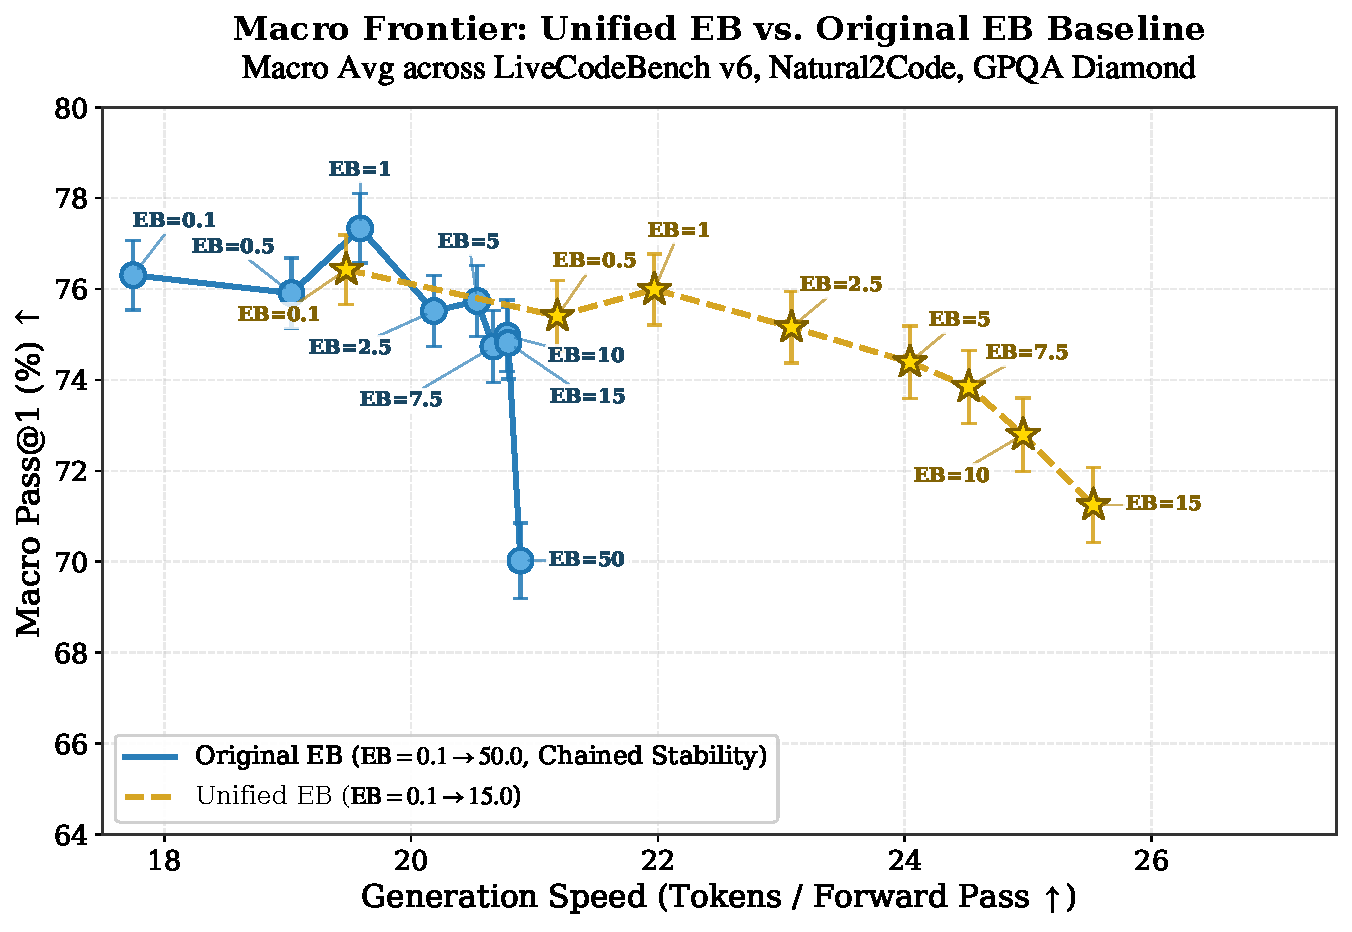
\includegraphics[width=\linewidth]{images/fig_macro_frontier_original_vs_unified.pdf}
        \caption{Original vs.\ unified stopping.}
        \label{fig:unified-vs-orig}
    \end{subfigure}
    \hfill
    \begin{subfigure}[b]{0.49\textwidth}
        \centering
        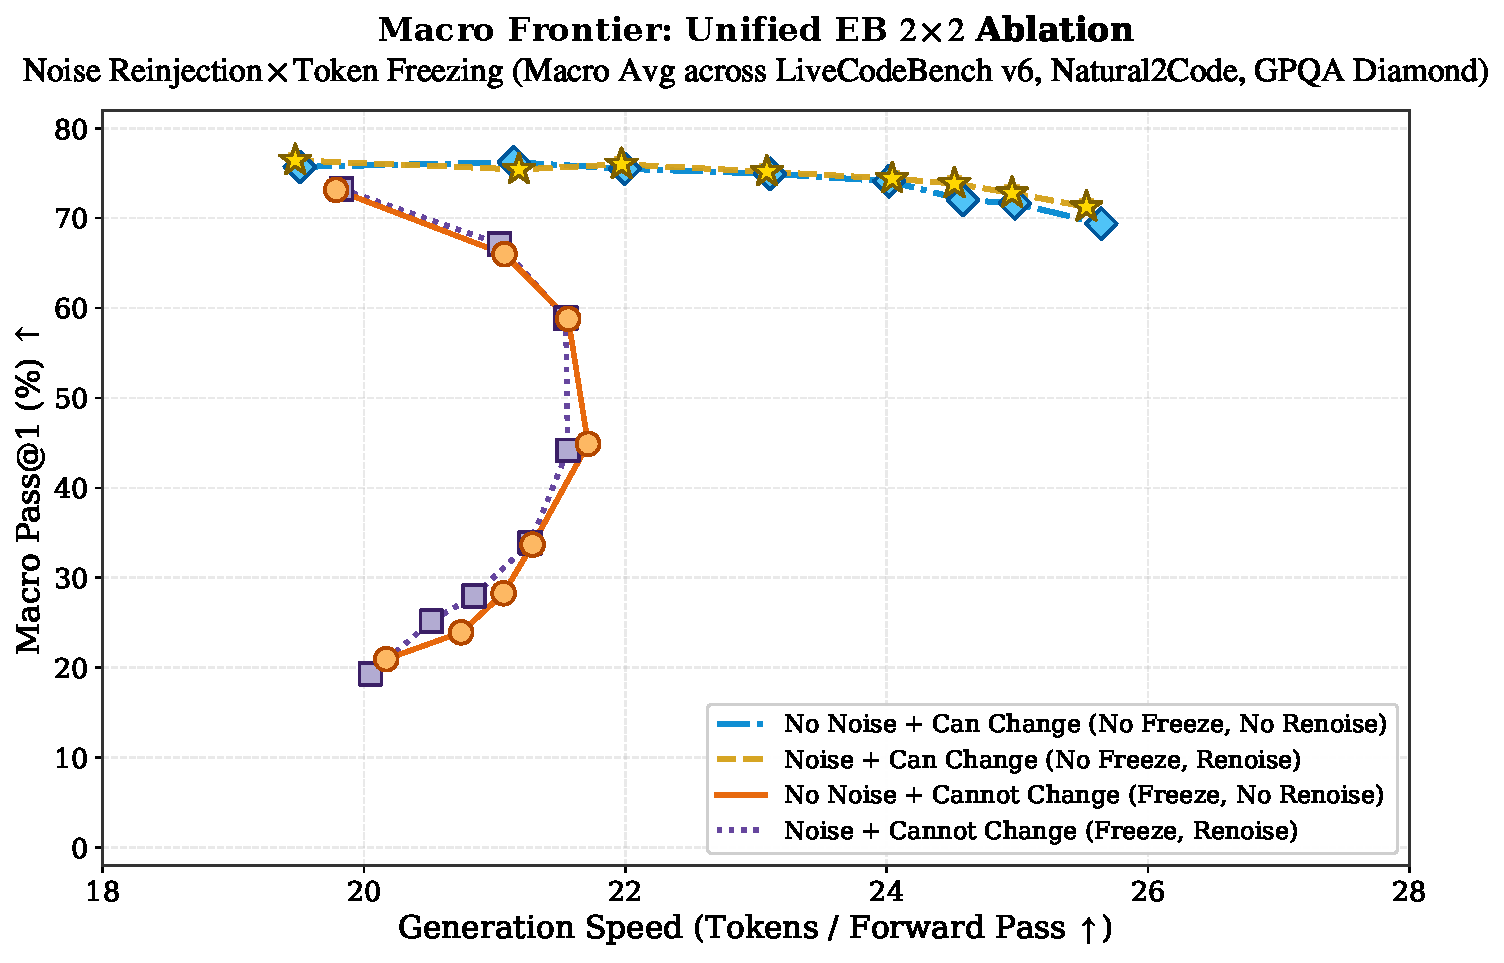
\includegraphics[width=\linewidth]{images/fig_macro_frontier_unified_ablation_2x2.pdf}
        \caption{Frozen vs.\ base EB sampler.}
        \label{fig:frozen-eb-frontier}
    \end{subfigure}

    \vspace{6pt}

    \begin{subfigure}[b]{\textwidth}
        \centering
        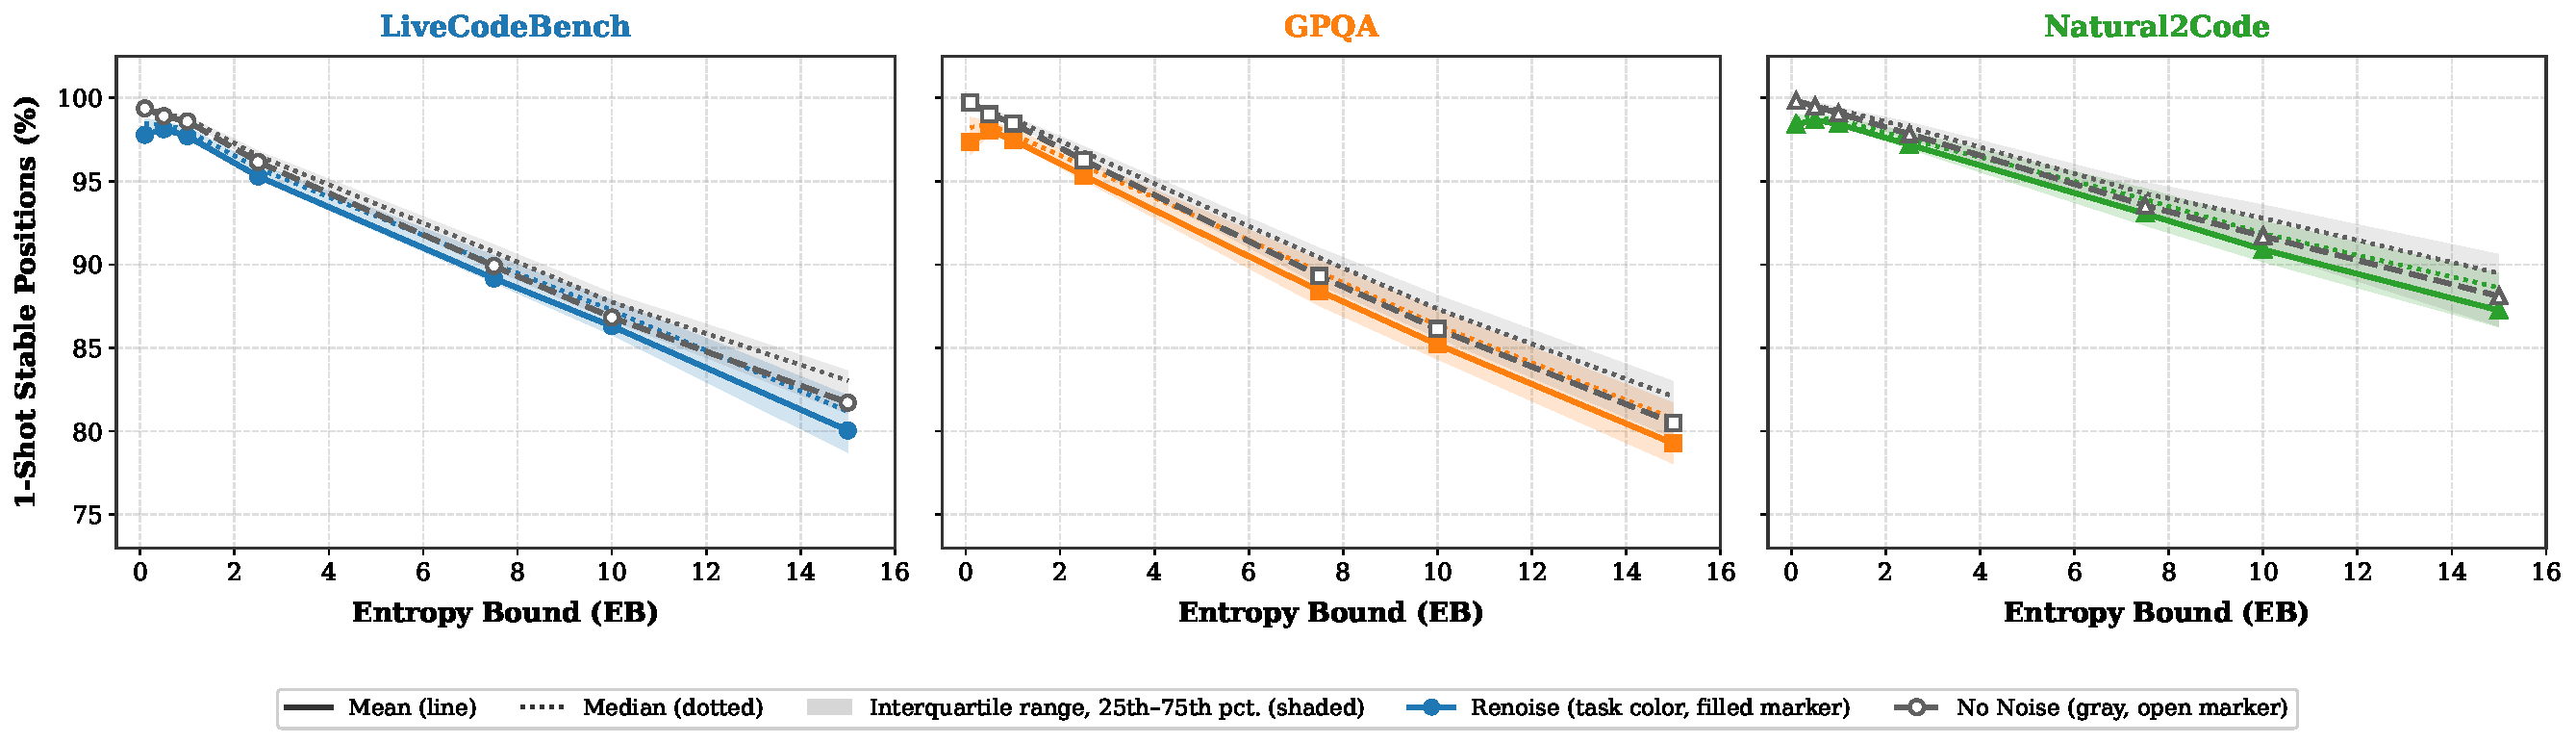
\includegraphics[width=\linewidth]{images/fig_1shot_stability_1x2_row.pdf}
        \caption{Stability of accepted tokens.}
        \label{fig:self-correct}
    \end{subfigure}
    \caption{\textbf{(a)} The unified stopping criterion matches the original at a slight speedup. \textbf{(b)} Pareto frontier of the modified EB sampler: larger entropy bounds trade performance for throughput, and the frozen variant degrades much faster than the base version, showing that the flexibility of the uniform diffusion process drives the frontier. \textbf{(c)} Accepted tokens are revised more often at higher entropy bounds (in both argmax and sampled-token stability), independent of renoising.}
    \label{fig:eb-frontiers}
\end{figure}
\paragraph{Setup}
We focus on the EB sampler, as it is the default sampler used in \citet{team2026diffusiongemma}.
Our goal is to determine if DiffusionGemma exhibits self-correcting behavior, and whether this is driven by the model or the sampler.
To do this, we measure the macro-average of AIME 2026, LCB v6, and HumanEval.
We introduce two interventions axis to investigate these questions: whether accepted tokens are "frozen" as in masked diffusion, and whether rejected tokens are renoised per the original sampler.

\paragraph{Frozen EB Sampler}
To do this, we first introduce a "freezing" variant of the EB sampler, where positions that are accepted under the EB rule cannot be changed later on, similar to masked diffusion. 
We refer to the original EB sampler as "unconstrained", as any position can be changed regardless of whether it was already accepted under the EB rule.

\paragraph{No Noise}
To determine whether the self-correction is driven by the sampler, we additionally introduce a version of the sampler that does not renoise the rejected positions as done in the original sampler. 
If there is no additional noise injection, then the model must be able to directly correct mistakes as opposed to relying on the noise to reset incorrect positions.
This can be thought of as an Euler sampler, as it is strictly interpolating between a uniform random sample and the final sample.

\paragraph{Ablation}
Both the no noise and frozen EB sampler are orthogonal directions of intervention. Thus we ablate over all four combinations and show the results in Figure \ref{fig:frozen-eb-frontier}.
For each possible combination, we do a sweep over various entropy bound values to examine how they are affected by more relaxed thresholds. 
For the unconstrained variants, we also track the empirical frequencies of each position being altered during the denoising trajectory after the initial acceptance under the EB rule.
We show these position volatility metrics in Figure \ref{fig:self-correct}.



\paragraph{Results}
We observe that for each adaptive variant, the unconstrained sampler achieves a superior pareto frontier than the frozen sampler, and this gap increases with further relaxation of the thresholds.
Furthermore, the number of positions that change after initial acceptance increases with higher entropy thresholds, and is relatively unaffected by whether the sampler uses noise injection.
This indicates that 1) the model does rely on self correction, as removing this deteriorates performance at relaxed thresholds; and 2) the self-correcion is driven by the changes in the models posterior as opposed to renoising, as removing noise does not alter post-acceptance behavior.

\subsection{Autoregressive Acceptance Order}
Here we examine the acceptance order of DiffusionGemma across a range of different acceptance rules.
We observe that DiffusionGemma exhibits a sampling order strongly biased towards autoregressive generation.
This autoregressive bias results in many denoising slots within a canvas being "wasted" on tokens that have already converged.
As a result, a form of rolling sampler where the window moves incrementally through the sequence rather than block by block becomes increasingly appealing as a way to extend the pareto frontier.

\begin{figure}[tbp]
\centering
\begin{tikzpicture}[x=0.205cm, y=0.205cm]

\definecolor{cwinfill}{HTML}{9FE1CB}
\definecolor{cwinedge}{HTML}{0F6E56}
\definecolor{camber}{HTML}{E8A13C}
\definecolor{camberedge}{HTML}{A96A0B}
\definecolor{cwaste}{HTML}{C0553C}
\definecolor{cwasteedge}{HTML}{7A2E1C}
\definecolor{cnoise}{HTML}{D3D1C7}
\definecolor{cnoiseedge}{HTML}{888780}
\definecolor{cclean}{HTML}{FFFFFF}
\definecolor{ccleanedge}{HTML}{B4B4A9}
\definecolor{cframe}{HTML}{2B5E94}

\newcommand{\gridcell}[3]{%
  \ifcase#3\relax
  \or \fill[cwinfill!65, draw=cwinedge,   line width=0.3pt, rounded corners=0.5pt] (#1, -#2) rectangle ++(0.88, -0.88);
  \or \fill[camber!45,   draw=camberedge, line width=0.3pt, rounded corners=0.5pt] (#1, -#2) rectangle ++(0.88, -0.88);
  \or \fill[cwaste,      draw=cwasteedge, line width=0.3pt, rounded corners=0.5pt] (#1, -#2) rectangle ++(0.88, -0.88);
  \or \fill[cclean,      draw=ccleanedge, line width=0.3pt, rounded corners=0.5pt] (#1, -#2) rectangle ++(0.88, -0.88);
  \or \fill[cnoise,      draw=cnoiseedge, line width=0.3pt, rounded corners=0.5pt] (#1, -#2) rectangle ++(0.88, -0.88);
  \fi}

\newcommand{\gridrow}[4]{%
  \foreach \c in {0,...,23} {%
    \pgfmathtruncatemacro{\sty}{\c<#3 ? 4 : (\c<#4 ? 1 : 5)}%
    \pgfmathsetmacro{\xpos}{\c + #1}%
    \gridcell{\xpos}{#2}{\sty}%
  }}

\newcommand{\gridmarks}[4]{%
  \foreach \c in {#4} {%
    \pgfmathsetmacro{\xpos}{\c + #1}%
    \gridcell{\xpos}{#2}{#3}%
  }}

\newcommand{\keydenoise}{\begin{tikzpicture}[baseline=-0.5ex, x=0.30cm, y=0.30cm]
  \fill[cwinfill!65, draw=cwinedge, line width=0.3pt, rounded corners=0.5pt] (0,-0.5) rectangle ++(0.88,1);
\end{tikzpicture}}
\newcommand{\keyaccept}{
\begin{tikzpicture}[baseline=-0.5ex, x=0.30cm, y=0.30cm]
  \fill[camber!45, draw=camberedge, line width=0.3pt, rounded corners=0.5pt] (0,-0.5) rectangle ++(0.88,1);
\end{tikzpicture}}
\newcommand{\keywaste}{
\begin{tikzpicture}[baseline=-0.5ex, x=0.30cm, y=0.30cm]
  \fill[cwaste, draw=cwasteedge, line width=0.3pt, rounded corners=0.5pt] (0,-0.5) rectangle ++(0.88,1);
\end{tikzpicture}}
\newcommand{\keycache}{
\begin{tikzpicture}[baseline=-0.5ex, x=0.30cm, y=0.30cm]
  \fill[cclean, draw=ccleanedge, line width=0.3pt, rounded corners=0.5pt] (0,-0.5) rectangle ++(0.88,1);
\end{tikzpicture}}
\newcommand{\keyunadmitted}{
\begin{tikzpicture}[baseline=-0.5ex, x=0.30cm, y=0.30cm]
  \fill[cnoise, draw=cnoiseedge, line width=0.3pt, rounded corners=0.5pt] (0,-0.5) rectangle ++(0.88,1);
\end{tikzpicture}}

\node[anchor=west, font=\footnotesize\bfseries] at (0, 1.5) {(a) Block sampler, $b=8$: 19 passes};

\gridrow{0}{0}{0}{8}
\gridrow{0}{1}{0}{8}
\gridrow{0}{2}{0}{8}                     \gridmarks{0}{2}{2}{0,3}
\gridrow{0}{3}{0}{8} \gridmarks{0}{3}{3}{0,3}          \gridmarks{0}{3}{2}{1,2}
\gridrow{0}{4}{0}{8} \gridmarks{0}{4}{3}{0,1,2,3}      \gridmarks{0}{4}{2}{4,6}
\gridrow{0}{5}{0}{8} \gridmarks{0}{5}{3}{0,1,2,3,4,6}  \gridmarks{0}{5}{2}{5,7}
\gridrow{0}{6}{8}{16}
\gridrow{0}{7}{8}{16}
\gridrow{0}{8}{8}{16}                        \gridmarks{0}{8}{2}{8,11}
\gridrow{0}{9}{8}{16}  \gridmarks{0}{9}{3}{8,11}             \gridmarks{0}{9}{2}{9}
\gridrow{0}{10}{8}{16} \gridmarks{0}{10}{3}{8,9,11}          \gridmarks{0}{10}{2}{10,13}
\gridrow{0}{11}{8}{16} \gridmarks{0}{11}{3}{8,9,10,11,13}    \gridmarks{0}{11}{2}{12,14}
\gridrow{0}{12}{8}{16} \gridmarks{0}{12}{3}{8,9,10,11,12,13,14} \gridmarks{0}{12}{2}{15}
\gridrow{0}{13}{16}{24}
\gridrow{0}{14}{16}{24}
\gridrow{0}{15}{16}{24}                          \gridmarks{0}{15}{2}{16,19}
\gridrow{0}{16}{16}{24} \gridmarks{0}{16}{3}{16,19}              \gridmarks{0}{16}{2}{17,18}
\gridrow{0}{17}{16}{24} \gridmarks{0}{17}{3}{16,17,18,19}        \gridmarks{0}{17}{2}{20,22}
\gridrow{0}{18}{16}{24} \gridmarks{0}{18}{3}{16,17,18,19,20,22}  \gridmarks{0}{18}{2}{21,23}

\foreach \x in {7.94, 15.94} {
  \draw[cframe, dashed, line width=0.4pt] (\x, 0.3) -- (\x, -19.2);
}
\node[anchor=east, font=\scriptsize] at (-0.5, -0.44) {$t=1$};
\node[anchor=east, font=\scriptsize] at (-0.5, -18.44) {$t=19$};

\node[anchor=west, font=\footnotesize\bfseries] at (29.5, 1.5) {(b) Rolling sampler, $w=8$: 13 passes};

\gridrow{29.5}{0}{0}{8}
\gridrow{29.5}{1}{0}{8}
\gridrow{29.5}{2}{0}{8}                          \gridmarks{29.5}{2}{2}{0,3}
\gridrow{29.5}{3}{1}{9}   \gridmarks{29.5}{3}{3}{3}          \gridmarks{29.5}{3}{2}{1,2}
\gridrow{29.5}{4}{4}{12}                         \gridmarks{29.5}{4}{2}{4,6}
\gridrow{29.5}{5}{5}{13}  \gridmarks{29.5}{5}{3}{6}          \gridmarks{29.5}{5}{2}{5,7,8}
\gridrow{29.5}{6}{9}{17}                         \gridmarks{29.5}{6}{2}{9,12}
\gridrow{29.5}{7}{10}{18} \gridmarks{29.5}{7}{3}{12}         \gridmarks{29.5}{7}{2}{10,11}
\gridrow{29.5}{8}{13}{21}                        \gridmarks{29.5}{8}{2}{13,14,17}
\gridrow{29.5}{9}{15}{23} \gridmarks{29.5}{9}{3}{17}         \gridmarks{29.5}{9}{2}{16,18}
\gridrow{29.5}{10}{15}{23} \gridmarks{29.5}{10}{3}{16,17,18} \gridmarks{29.5}{10}{2}{15,19}
\gridrow{29.5}{11}{20}{24}                       \gridmarks{29.5}{11}{2}{20,22}
\gridrow{29.5}{12}{21}{24} \gridmarks{29.5}{12}{3}{22}       \gridmarks{29.5}{12}{2}{21,23}

\node[anchor=east, font=\scriptsize] at (29.0, -0.44) {$t=1$};
\node[anchor=east, font=\scriptsize] at (29.0, -12.44) {$t=13$};

\node[anchor=north, font=\scriptsize, inner sep=0pt] at (26.7, -20.4) {%
  \begin{tabular}{@{}l@{~}l@{\hspace{1.8em}}l@{~}l@{\hspace{1.8em}}l@{~}l@{}}
    \keydenoise & denoising slot   & \keyaccept     & accepted on this pass &
    \keywaste   & wasted: re-denoised while waiting \\[2.5pt]
    \keycache   & in the KV cache  & \keyunadmitted & not yet admitted      &
                &                                    \\
  \end{tabular}};

\end{tikzpicture}
\caption{\textbf{Where the denoising slots go.} Both samplers denoise a
width-$8$ window per pass in the same order, and the colours are those of
Figure~\ref{fig:algorithm-concept}: teal = still denoising, amber = accepted
on this pass, white = already encoded and in the KV cache, gray = not yet
admitted.  Brick marks a slot spent re-denoising a position that was already
accepted but is still waiting for its prefix, that is, wasted work.
\textbf{(a)} The block sampler appends only once the block is fully resolved,
so converged positions idle and each block re-pays warm-up.  \textbf{(b)} The
rolling sampler appends the accepted prefix immediately and admits fresh
positions in its place, wasting far fewer slots.}
\label{fig:block-vs-rolling}
\end{figure}


\paragraph{Defining Redundant Computations}
Here we define what constitutes a redundant computation.
Our goal is to measure the computations that could be conceivable omitted without drastically impacting the model's behavior.
Thus we define wasted denoising slots as positions that have already converged and are part of a contiguous prefix that could be appended to the KV cache.
We illustrate this definition in Figure \ref{fig:block-vs-rolling}, against the ideal sampler that commits them to the KV cache and avoids redundant denoising steps.

\begin{figure}[tbp]
    \centering
    \begin{subfigure}[b]{\textwidth}
        \centering
        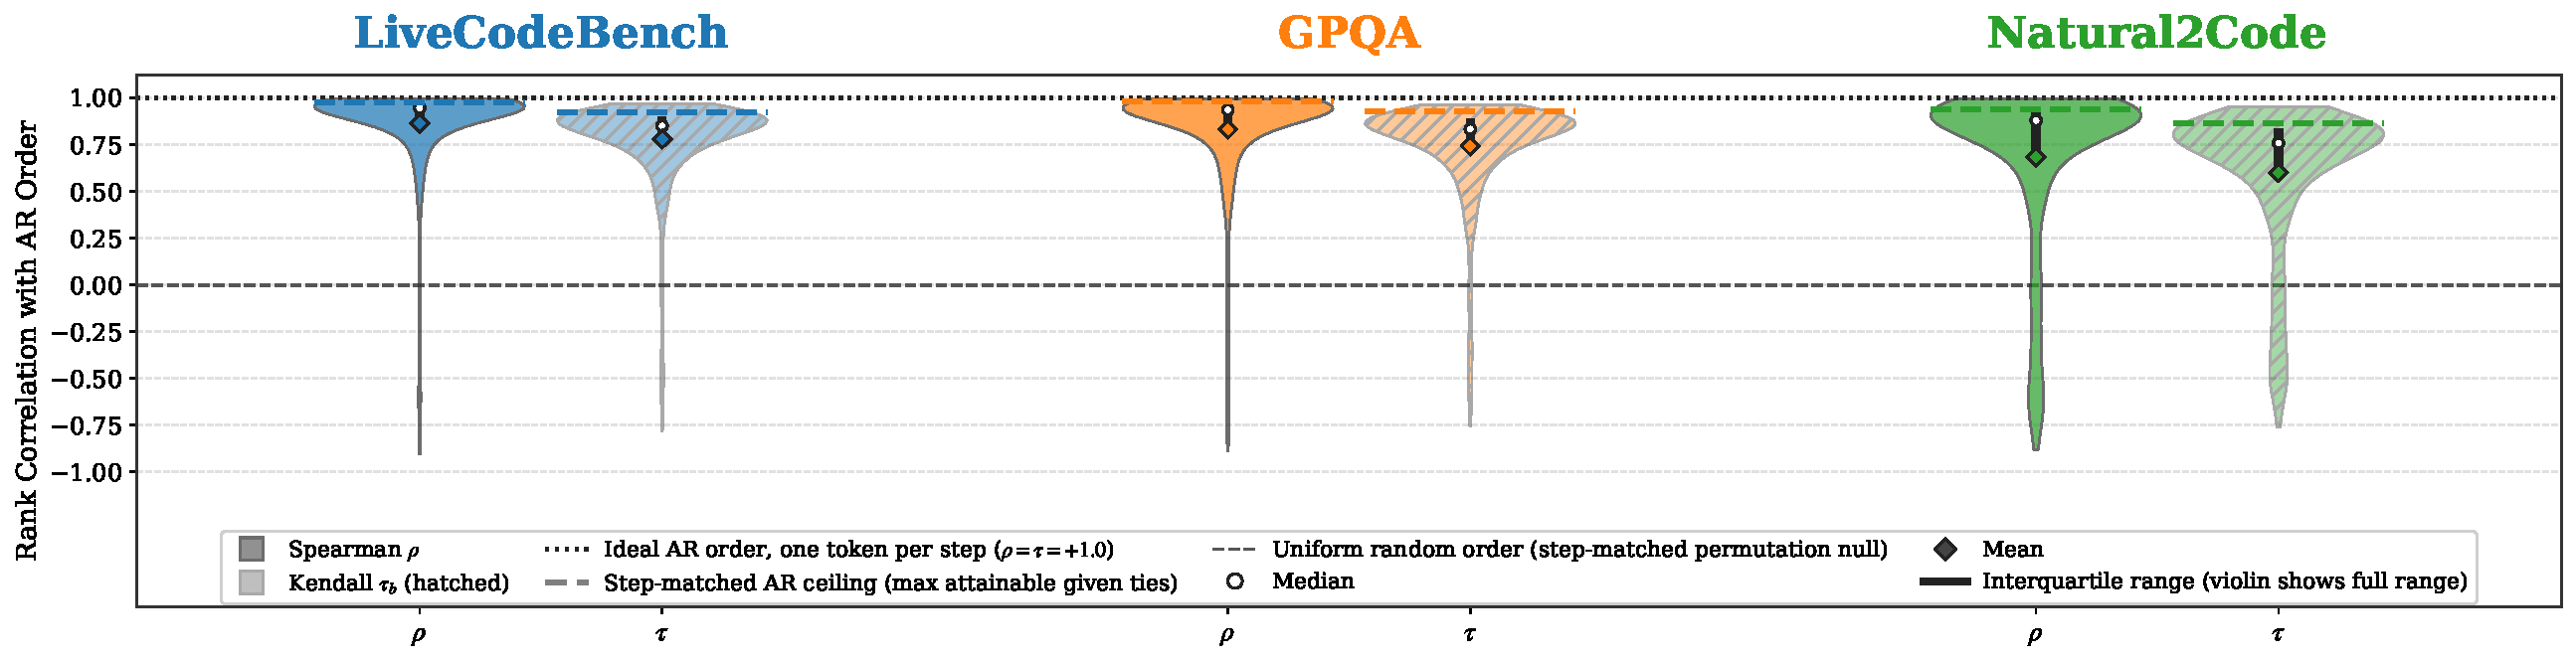
\includegraphics[width=\linewidth]{images/fig_ar_order_correlation_eb0.1_renoise.pdf}
        \caption{Commitment order vs.\ AR order.}
        \label{fig:ar-order-correlation}
    \end{subfigure}

    \vspace{6pt}

    \begin{subfigure}[b]{\textwidth}
        \centering
        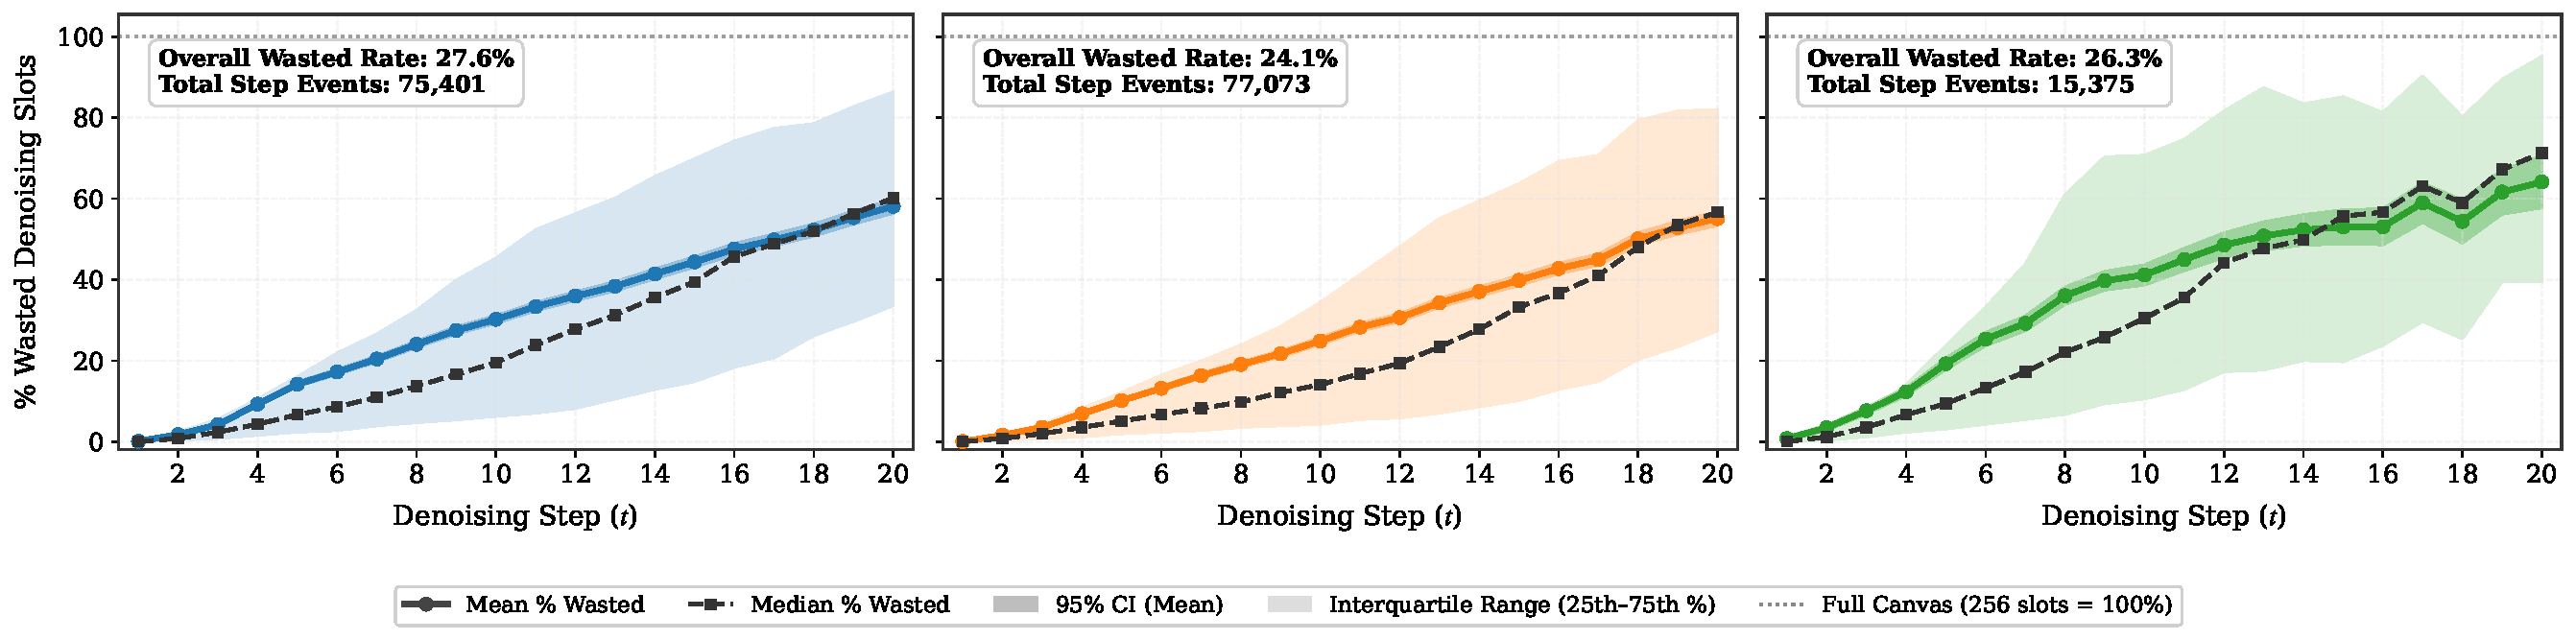
\includegraphics[width=\linewidth]{images/wasted_canvas_slots_lcb_gpqa_n2c.pdf}
        \caption{Wasted denoising slots.}
        \label{fig:wasted-slots}
    \end{subfigure}
    \caption{\textbf{(a)} Spearman $\rho$ and Kendall $\tau$ between the commitment order of the DiffusionGemma EB sampler and the AR generation order; across all tasks the sampler is strongly biased towards left-to-right order. \textbf{(b)} Number of wasted denoising slots averaged across canvases for AIME, LCB and HumanEval. For a given sampling step, a slot is wasted if it belongs to a contiguous prefix that has already converged to its final token. Past 10 denoising steps, over half of the canvas slots are wasted.}
    \label{fig:wasted}
\end{figure}

\paragraph{Experimental Setup}
We run the unified EB sampler on LCB v6, GPQA Diamond and Natural2Code. We track the trajectories of each denoising block, and consider a position as converged when it realizes the value that ends up being committed to the KV cache.

\paragraph{Results}
In Figure \ref{fig:ar-order-correlation}, we observe that the convergence orderign of positions is very correlated with left-to-right order. This explains the behavior of wasted denoising slots in Figure \ref{fig:wasted-slots}, where we observe that the percentage of wasted slots increases monotonically during the denoising trajectory.  

This has been observed previously by \citep{asaria2026neither}, where they observe the autoregressive bias of the DiffusionGemma sampler. 
This is not a model specific quirk: this aligns with many general observations of the sampling behavior for confidence-based samplers for large scale diffusion language models. 
\citet{kim2026interface} demonstrates that confidence based samplers tend to generate samples that are very similar to those produced by left-to-right autoregressive order. 
Other works demonstrate that the ordering itself is highly left to right and provide various explanations for why \citep{gong2026diffucoder, lu2026adablock, yao2026decoding}.

\paragraph{Self Correcting or Rolling?}
Through studying adaptive samplers for uniform diffusion, we observe the following:
\begin{enumerate}
    \item DiffusionGemma exhibits self correcting behavior that allows for a strictly better pareto frontier with relaxed thresholds. 
    \item DiffusionGemma also exhibits a strong autoregressive bias, which points towards a rolling mechanism as a simple means of extending the frontier.
\end{enumerate}

These two mechanisms for extending the frontier are orthogonal: self correction requires flexibility, whereas the rolling sampler would depend on token stability. 
However, it is unclear how these two orthogonal mechanisms for extending the frontier compare.
In the next section, we introduce a rolling diffusion sampler that incrementally commits tokens to the KV cache to investigate this question.